\documentclass[11pt]{article}
\usepackage[margin=1in]{geometry}
\usepackage[T1]{fontenc}
\usepackage{lmodern}
\usepackage{booktabs}
\usepackage{amsmath}
\usepackage{xcolor}
\usepackage{enumitem}
\usepackage[hidelinks]{hyperref}
\usepackage{caption}
\usepackage{float}
\usepackage{tikz}
\usetikzlibrary{positioning,arrows.meta}
\usepackage{pgfplots}
\pgfplotsset{compat=1.16}
\definecolor{cA}{HTML}{2A78D6}
\definecolor{cB}{HTML}{C8641B}
\definecolor{cG}{HTML}{4A3AA7}

\newcommand{\todo}[1]{\textcolor{red}{\textbf{[TODO: #1]}}}
\setlist{itemsep=2pt,topsep=3pt}

\title{Exact Top-$k$ Learned Sparse Retrieval on the GPU:\\
Two Strategies over a Range-Partitioned Bit-Packed Index}
\author{Arnav Gupta \quad Vaibhav Chaudhari \quad Parva Patel\\[4pt]
\small CSCI-GA 3033-025: GPU Architecture and Programming, New York University}
\date{Fall 2026}

\begin{document}
\maketitle

% =====================================================================
\begin{abstract}
Learned sparse retrieval models like SPLADE represent queries and documents as sparse vectors over a vocabulary, and a top-k retrieval returns $k$ documents with the highest dot product with the query. Doing this \emph{exactly} over millions of documents is the first stage of modern search and question-answering pipelines, and its latency bounds the whole system. The problem is usually considered a poor fit for a naive GPU implementation with posting lists being irregular, the number of candidate documents being huge, and the final top-$k$ selection itself being expensive. We introduce a range-partitioned, bit-packed inverted index in which every GPU thread block scores one contiguous range of documents entirely in shared memory. On this base, we build two complementary strategies:
\begin{itemize}
\item \textbf{Strategy A} scores every range and selects the top $k$ with radix-based algorithms, so
  its cost barely grows with $k$;
\item \textbf{Strategy B} uses upper bounds to skip whole ranges that cannot reach the top $k$.
\end{itemize}
On the full 8.8M-passage MS~MARCO collection on an RTX~4070, both return exact results. Strategy B is fastest at $k=10$ (0.205\,ms per query), and Strategy A is fastest at $k=100$ and
$k=1000$ (0.455 and 0.834\,ms). Against a same-hardware adaptation of the recent GPUSparse system,
the best strategy at each depth is 7.5--29$\times$ faster.
\end{abstract}

% =====================================================================
\section{Introduction}

In learned sparse retrieval (LSR), a neural encoder maps each document and each query to a sparse vector of term weights over a vocabulary of about 30{,}000 terms \cite{splade,spladepp}. The score of a document is the dot product
\[
  s(q,d) \;=\; \sum_{t \in q \cap d} w_q(t)\, w_d(t),
\]
and retrieval returns the top $k$ highest-scoring documents. Document vectors are encoded once, offline, and stored as an inverted index: for every term, the list of documents containing it together with their weights (\emph{impacts}). At query time only the query's terms (typically 20--60) are read.

First-stage retrieval feeds every later stage, such as re-rankers and retrieval-augmented generation, so its latency is paid on every request. \emph{Exact} retrieval matters because approximate methods trade recall for speed in ways that are hard to bound. The depth $k$ also varies by use: $k=10$ for direct answers, $k=1000$ when a re-ranker follows. A good system
has to be fast across that whole range.

This is difficult to do on a GPU. SPLADE posting lists are long and highly skewed. The number of
documents a query touches is in the millions, and selecting the top $k$ from them needs either a large
score array or a careful parallel selection. CPU engines rely on sequential dynamic pruning (WAND,
MaxScore, Block-Max) \cite{wand,maxscore,bmw}, whose data-dependent control flow maps poorly onto GPU
threads.

\textbf{We} design an inverted index cut into fixed-size \emph{ranges} of document IDs,
so that each GPU thread block scores one range entirely in shared memory. On this foundation we build
two strategies:
\begin{itemize}
\item \textbf{Strategy A} makes exhaustive scoring fast at every depth, with threshold-filtered
  candidates, radix-select top-$k$, latency-hiding decoding and a parallel radix-select merge;
\item \textbf{Strategy B} skips ranges using per-range upper bounds, refined by a two-half filter.
\end{itemize}
We compare both against each other and against GPU and CPU baselines, under one exactness contract and
one statistical timing protocol.

% =====================================================================
\section{Literature Survey}

\paragraph{Learned sparse retrieval.} SPLADE \cite{splade} and its successors \cite{spladepp} learn term
weights and expansion terms with a BERT masked-language-model head. The resulting sparse vectors work
with inverted indexes. We use the public quantized SPLADE CoCondenser-EnsembleDistil encoding of
MS~MARCO \cite{msmarco}, distributed in the Common Index File Format \cite{ciff} by the PISA project
\cite{pisa}.

\paragraph{Dynamic pruning on the CPU.}
\begin{itemize}
\item WAND \cite{wand} and MaxScore \cite{maxscore} skip documents whose upper bound cannot beat the
  current $k$-th score $\theta$.
\item Block-Max WAND \cite{bmw} stores a maximum impact per block of postings to tighten those bounds.
\item Block-Max Pruning (BMP) \cite{bmp}, designed for learned sparse vectors, partitions documents into
  blocks with per-term block maxima, visits blocks in bound order and stops when the bound falls below
  $\theta$.
\end{itemize}
\emph{Limitation:} these algorithms are sequential per query and branch-heavy, which does not map onto
thousands of GPU threads.

\paragraph{Retrieval and pruning on GPUs.}
\begin{itemize}
\item Gaioso et al.\ \cite{gaiosowand} parallelise WAND on GPUs by partitioning the index by document
  ranges and sharing the threshold $\theta$ between thread blocks.
\item Huang et al.\ \cite{huangbmw} run Block-Max WAND per thread over
  compressed lists.
\item GPUSparse \cite{gpusparse} keeps a SPLADE inverted index resident on one GPU, scores exhaustively
  with a scatter-add over posting lists, then selects the top $k$. It reports 1.27\,ms per query at
  batch 500 and 9.6\,ms for a single query on an H100.
\end{itemize}
\emph{Limitation:} GPUSparse scores every document into a collection-sized array, so its single-query
cost is high, and its upper-bound pruning did not reduce latency on SPLADE. The thread-level WAND
traversals suffer from load imbalance.

\paragraph{Related problems with similar challenges.}
\begin{itemize}
\item \emph{Sparse matrix--vector products} face the same irregularity. Merge-based SpMV
  \cite{mergespmv} balances work by splitting rows and non-zeros evenly; bucket-based approaches group
  outputs by row range, which is analogous to our ranges.
\item \emph{GPU integer compression} with tile-based bit packing \cite{gpufor} decodes in parallel
  without sequential dependencies, which informed our encoding; GPU-VByte decoding is another
  GPU-oriented approach \cite{zahrangpuvbyte}.
\item \emph{GPU top-$k$ selection:} bitonic top-$k$ \cite{bitonictopk}, warp-level selection in Faiss
  \cite{faiss}, radix-based selection (AIR Top-K \cite{airtopk}, RadiK \cite{radik}) and
  delegate-based filtering (Dr.~Top-k \cite{drtopk}).
\end{itemize}

\paragraph{Why a new design.} None of these combines (i) exact results under a fixed integer contract,
(ii) low single-query latency on a consumer GPU, and (iii) good behaviour from $k=10$ to $k=1000$.

% =====================================================================
\section{Proposed Idea}

\subsection{Exactness contract}
Both strategies return results identical to a CPU reference under one contract:
\begin{itemize}
\item document impacts are uint8;
\item query weights are quantised with a cap of 32;
\item scores are exact integer sums;
\item every passage is eligible, including those scoring 0;
\item results are ordered by score descending, then original passage ID ascending.
\end{itemize}

\subsection{Common foundation: a range-partitioned bit-packed index}
\paragraph{Layout.} Documents are cut into ranges of $W$
consecutive document IDs. Each (term, range) pair that has postings becomes one \emph{block}, and blocks
are stored term-major. The index consists of:
\begin{itemize}
\item \texttt{encoded}: each block's in-range document positions, bit-packed at the block's own width
  (at most $\lceil\log_2 W\rceil$ bits). Storing positions rather than gaps lets every posting be
  decoded independently, rather than requiring a prefix sum: the $j$-th value of a block starts at bit $\mathit{start} + j \cdot
  \mathit{width}$;
\item \texttt{impacts}: one byte per posting, in the same order;
\item per-block metadata: start bit, impact offset, count, width, and the block's range;
\item a per-term lookup into the sorted list of ranges in which the term occurs;
\item the range boundaries and a map from internal document numbers to original passage IDs.
\end{itemize}
The index is built offline and loaded onto the GPU once.

\paragraph{Execution model.} One kernel launch processes one query, and thread block $r$ scores range $r$
(Figure~\ref{fig:model}):
\begin{enumerate}
\item for each query term, binary-search the term's range list for $r$ and copy that block's metadata
  into shared memory;
\item zero a shared accumulator \texttt{scores[W]};
\item stride over the range's combined list of query postings (all query terms together), extract each
  position with one or two 32-bit loads and shifts, load the impact, and \texttt{atomicAdd} the
  weighted impact into shared memory;
\item select the range's local top $k$ and write the candidates to global memory;
\item the last block to finish, detected with a global atomic counter after a memory fence, merges all
  candidates and writes the final top $k$.
\end{enumerate}
\begin{figure}[H]\centering
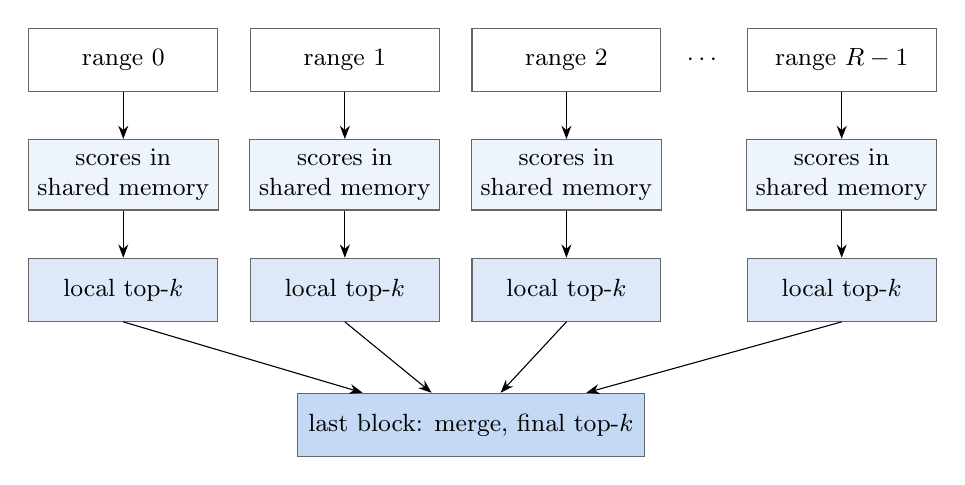
\begin{tikzpicture}[font=\small,>=Stealth,b/.style={draw=black!60,minimum height=8mm,minimum width=24mm,align=center}]
\node[b] (r0) {range 0};\node[b,right=4mm of r0] (r1) {range 1};\node[b,right=4mm of r1] (r2) {range 2};\node[right=2mm of r2] (dd) {$\cdots$};\node[b,right=2mm of dd] (rn) {range $R-1$};
\foreach \n in {r0,r1,r2,rn}{\node[b,below=6mm of \n,fill=cA!8] (s\n) {scores in\\shared memory};\node[b,below=6mm of s\n,fill=cA!16] (t\n) {local top-$k$};\draw[->] (\n)--(s\n);\draw[->] (s\n)--(t\n);}
\node[b,below=9mm of tr1,xshift=16mm,fill=cA!28,minimum width=44mm] (m) {last block: merge, final top-$k$};
\foreach \n in {r0,r1,r2,rn} \draw[->] (t\n.south)--(m);
\end{tikzpicture}
\caption{Execution model: one thread block scores one range of documents in shared memory, and the last block to finish merges the candidates. Strategy B takes only the ranges it could not skip.}
\label{fig:model}
\end{figure}
Each block's accumulator covers only $W$ documents, so it fits in shared memory and no
collection-sized array is needed.

\subsection{Strategy A: exhaustive range scoring with radix-based selection}
Strategy A scores every range and makes selection and merging cheap at any depth, using four techniques:
\begin{enumerate}
\item \textbf{Shared threshold on candidates.} After its local selection, a range holding at least $k$
  documents raises a global threshold $\theta$ to its own $k$-th score with \texttt{atomicMax}. This is
  safe: that range alone proves that $k$ documents score at least that much. Each range then writes
  only candidates scoring $\geq\theta$, with ties kept. This adopts the shared-threshold idea of
  \cite{gaiosowand}. At $k=10$ it reduces the candidates written by 95\% and those reaching the final
  merge by over 99\%.
\item \textbf{Radix-select local top-$k$.} Each block forms 64-bit keys (score, then the document's
  in-range ID rank, so ties stay exact) and runs an 8-bit radix select \cite{radik,airtopk}: histogram
  the current digit in shared memory, find the bucket containing the $k$-th key, accept everything
  above it, and recurse only into that bucket. The winners are then ordered with a bitonic sort. The cost
  depends on $W$, not on $k$.
\item \textbf{Latency-hiding decode.} Each thread computes addresses and issues the memory loads for four
  postings before using any of them, so their global-memory latencies overlap rather than add up.
\item \textbf{Parallel merge by compaction and radix select.} The last block compacts all surviving
  candidates from every range into one array, with a prefix sum over per-range counts. It then runs the
  same radix select over 64-bit keys (score, then the document's global ID rank) and sorts the winners.
  The merge thus uses all of the block's threads in a fixed number of passes, instead of about $k$
  serial rounds.
\end{enumerate}

\subsection{Strategy B: bound-based range pruning with a two-half filter}
Strategy B scores only the ranges that can contain a top-$k$ document. It needs one extra table, built when the
index is loaded: the largest impact of every (term, range) block, and, for the two-half filter, the largest
impact in each half of the block. A query runs as a fixed sequence of kernels on one stream, with no round trip
to the host in between:
\begin{enumerate}
\item \textbf{Range bounds.} The bound of a range is $\sum_t w_q(t)\cdot\max_{d\in\text{range}} w_d(t)$, so no
  document in it can score more. The kernel goes term by term: the blocks of one term are contiguous in memory,
  and each thread adds (query weight $\times$ block maximum) to its range's bound with \texttt{atomicAdd}. Our
  first version used one thread per range with a binary search per term. Changing only this step made the whole
  query 1.36$\times$ faster ($W=256$, $k=10$).
\item \textbf{Seed selection.} One block picks the 64 ranges with the largest bounds, by radix select with 12-bit
  digits; ties go to the lower range number.
\item \textbf{Seed scoring.} The seeds are scored exactly. $\theta$ is the $k$-th best score among their
  documents, or 0 if they hold fewer than $k$ documents.
\item \textbf{Pruning and the two-half filter.} A range whose bound is below $\theta$ is dropped. For each
  remaining range, one warp computes a bound for each half (128 documents) and drops the range if both are below
  $\theta$. This costs a lookup per query term, but only for ranges that the first bound could not remove.
\item \textbf{Scoring.} The surviving ranges go on a work list. Thread blocks stay resident and take ranges from
  it with an atomic counter, so a skipped range costs no block launch. The scoring of a range follows the
  common execution model.
\item \textbf{Merge.} A range whose best document is below $\theta$ writes no list, and single candidates below
  $\theta$ are invalidated. The last block merges the remaining lists, picking the top $k$ one document at a
  time. This last part is simple, and it is what limits Strategy B at large $k$.
\end{enumerate}

\paragraph{Why the result is exact.} When $\theta>0$, at least $k$ seeded documents score $\theta$ or more. A
document in a dropped range scores strictly less than $\theta$, so it cannot be in the top $k$. Ranges and
candidates that only equal $\theta$ are kept, because they can still win a tie on passage ID.

\paragraph{Design choices.}
\begin{itemize}
\item \textbf{Range size.} Smaller ranges give tighter bounds. With 64 seeds and $k=10$ the median query scores
  34.5\% of the ranges at $W=1024$, 16.2\% at $W=512$ and 6.3\% at $W=256$. We use $W=256$, although queries
  that prune badly then pay for many small ranges.
\item \textbf{Number of seeds.} With 64 seeds the median query scores at most 3 percentage points more of its
  postings than with the ideal threshold (the true $k$-th score), so we did not tune it further.
\item \textbf{Pruning or smaller ranges?} Small ranges alone do not help. Without pruning, $W=256$ is slower
  than $W=1024$ (0.33$\times$ the speed); pruning then makes it 5.1$\times$ faster.
\end{itemize}

\paragraph{Complementary strengths.} The strategies reduce different costs. Strategy B reduces the
amount of scoring, which dominates when $k$ is small and $\theta$ is high. Strategy A reduces the cost of
selection and merging, which dominates at larger $k$.

% =====================================================================
\section{Experimental Setup}

\paragraph{Machine.} All reported experiments ran on one machine (cuda5 CIMS machine):
\begin{itemize}
\item GPU: one NVIDIA GeForce RTX~4070 (Ada Lovelace, compute capability 8.9, 46 SMs, 12\,GB GDDR6X,
  504\,GB/s, 36\,MB L2);
\item CPU: two Intel Xeon E5-2650 v2 (2.60\,GHz), 16 cores in total;
\item memory: 64\,GB;
\item operating system: Red Hat Enterprise Linux 9.
\end{itemize}

\paragraph{Software.}
\begin{itemize}
\item CUDA 12.6 (\texttt{nvcc -O3 -arch=sm\_89}), g++ 11.5 with C++17, Nsight Systems and
  Nsight Compute for profiling;
\item the GPUSparse baseline: Python 3.12.7, PyTorch 2.6.0 (CUDA 12.6) and Triton 3.2.0.
\end{itemize}

\paragraph{Data.}
\begin{itemize}
\item MS~MARCO passage ranking \cite{msmarco}: 8,841,823 passages, encoded with SPLADE
  CoCondenser-EnsembleDistil, impacts quantised to uint8 and documents in graph-bisection order (CIFF
  file from the PISA project, verified by SHA-256).
\item Subsets of 100K and 1M passages, for the scaling experiment.
\item Queries: 500 queries from the MS~MARCO dev (small) set. We also used these 500 queries to choose designs and settings.
\end{itemize}

\paragraph{Timing protocol.}
\begin{itemize}
\item Batch size 1. The timed region runs from building the query on the host to receiving the ordered
  top-$k$ back on the host. Index building, loading and upload are excluded.
\item Each configuration runs as 3 separate processes, each with 3 warm-up and 20 measured rounds over
  all queries (10 rounds in the session that timed Strategy B at $k=100$ and $k=1000$). We report the median over the per-query, per-process medians.
\item Systems compared within one session are paired by (process, query), with the order rotated between
  processes. Ratios are geometric means with 95\% bootstrap intervals (10,000 draws).
\item Decision rules were fixed before timing. The GPU had to have no active process of another user
  before every process, and a process that overlapped another user's GPU activity was discarded and rerun.
  Idle processes of other users were allowed to stay resident.
\item Every timed output was checked against the CPU reference: all results reported are exact (one exception on the
  order of ties is named in Section~\ref{sec:batch}).
\end{itemize}

\paragraph{Baselines.}
\begin{itemize}
\item \textbf{GPUSparse} \cite{gpusparse}: the released code, adapted to the exactness contract above,
  in three variants: exact 64-bit integer scoring (U64), guarded single-precision scoring (FP32), and FP32 scoring
  with document weights stored as uint8 (FP32/uint8), which is the fastest. Above $k=128$ we only raised the
  adapter's limit on $k$.
\item \textbf{CPU:} an exact exhaustive scorer (single- and multi-threaded) and BMP \cite{bmp}.
\end{itemize}

% =====================================================================
\section{Experiments and Analysis}

\subsection{Latency on the full collection}
\begin{table}[H]
\centering
\caption{Median per-query latency (ms) and peak GPU memory, full collection (8.84M passages),
RTX~4070, batch 1, 500 queries. All results are exact. Best per column in bold. The rows come from several
sessions: GPUSparse U64/FP32 and Strategy A share one, FP32/uint8 has its own, and Strategy B has one for
$k=10$ and one for $k=100$ and $k=1000$.}
\label{tab:main}
\begin{tabular}{lrrrr}
\toprule
System & $k=10$ & $k=100$ & $k=1000$ & GPU memory\\
\midrule
GPUSparse, U64 & 6.903 & 6.950 & 7.425 & 8.4\,GB\\
GPUSparse, FP32 & 6.021 & 6.077 & 6.534 & 8.3\,GB\\
GPUSparse, FP32/uint8 & 5.884 & 5.950 & 6.414 & 5.3\,GB\\
\midrule
Strategy A & 0.403 & \textbf{0.455} & \textbf{0.834} & 3.3--3.4\,GB\\
Strategy B & \textbf{0.205} & 0.576 & 3.080 & 5.1--5.9\,GB\\
\bottomrule
\end{tabular}
\end{table}

\begin{table}[H]
\centering
\caption{The slowest queries: p99 latency (ms) of the systems in Table~\ref{tab:main}.}
\label{tab:tail}
\begin{tabular}{lrrr}
\toprule
System & $k=10$ & $k=100$ & $k=1000$\\
\midrule
GPUSparse, FP32/uint8 & 8.571 & 8.636 & 9.115\\
Strategy A & \textbf{0.648} & \textbf{0.718} & \textbf{1.416}\\
Strategy B & 1.320 & 2.777 & 22.921\\
\bottomrule
\end{tabular}
\end{table}

\paragraph{Against GPUSparse.}
\begin{itemize}
\item \textbf{Strategy A} is 14.4$\times$ / 12.8$\times$ / 7.5$\times$ faster than the fastest GPUSparse variant
  (FP32/uint8) at $k=$ 10 / 100 / 1000, with about 63\% of its GPU memory.
\item \textbf{Strategy B} is about 29$\times$ / 10$\times$ / 2.1$\times$ faster than FP32/uint8
\item GPUSparse's latency barely depends on $k$ (+7.6\% for U64 and +9.0\% for FP32/uint8 from $k=10$ to 1000) because it
  always scores the whole collection into one array before selecting. Both strategies avoid that array,
  because each thread block scores its range in shared memory.
\end{itemize}

\begin{figure}[H]\centering
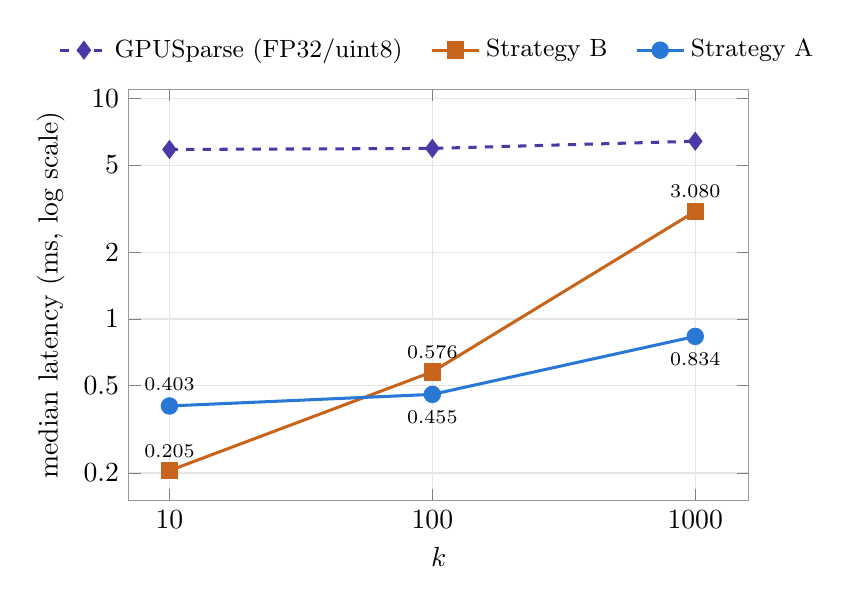
\begin{tikzpicture}\begin{axis}[width=.78\linewidth,height=6.8cm,xmode=log,ymode=log,xtick={10,100,1000},xticklabels={10,100,1000},ytick={0.2,0.5,1,2,5,10},yticklabels={0.2,0.5,1,2,5,10},minor tick style={draw=none},xlabel={$k$},ylabel={median latency (ms, log scale)},xmin=7,xmax=1600,ymin=.15,ymax=11,grid=major,grid style={black!10},axis line style={black!40},legend columns=3,legend style={draw=none,font=\small,at={(.5,1.04)},anchor=south,/tikz/every even column/.append style={column sep=8pt}},legend cell align=left,every axis plot/.append style={line width=1.1pt,mark size=2.6pt}]
\addplot[cG,mark=diamond*,dashed,mark options={solid}] coordinates{(10,5.884)(100,5.950)(1000,6.414)};\addlegendentry{GPUSparse (FP32/uint8)}
\addplot[cB,mark=square*,nodes near coords,point meta=explicit symbolic,every node near coord/.append style={font=\scriptsize,text=black,anchor=south,yshift=1pt}] coordinates{(10,.205)[0.205](100,.576)[0.576](1000,3.080)[3.080]};\addlegendentry{Strategy B}
\addplot[cA,mark=*,nodes near coords,point meta=explicit symbolic,every node near coord/.append style={font=\scriptsize,text=black,anchor=north,yshift=-2pt}] coordinates{(10,.403)[](100,.455)[0.455](1000,.834)[0.834]};\addlegendentry{Strategy A}
\node[font=\scriptsize,anchor=south,yshift=2pt] at (axis cs:10,.403) {0.403};
\end{axis}\end{tikzpicture}
\caption{Median latency against $k$ (log scales), full collection, 500 queries. The values are those of Table~\ref{tab:main}; the systems come from several sessions.}
\label{fig:depth}
\end{figure}

\paragraph{Strategy A against Strategy B.}
\begin{itemize}
\item At $k=10$, Strategy B is about 2$\times$ faster. This is because Strategy B, with a high threshold, scores only a
  small fraction of the ranges, while Strategy A scores all of them.
\item At $k=100$ and $k=1000$ (Figure~\ref{fig:depth}), Strategy A is 1.29$\times$ and 4.32$\times$ faster (paired, same
  session). As $k$ grows, $\theta$ falls, Strategy B keeps more ranges, and its selection and merge
  grow with $k$. Strategy A's grow very little: from $k=10$ to $k=1000$ its latency only doubles, while
  Strategy B's grows 15$\times$.
\item Strategy A also has the shorter tail at every depth (Table~\ref{tab:tail}). Strategy B's slowest queries are
  those whose bounds prune little.
\end{itemize}

\subsection{Where Strategy A spends its time}
\begin{itemize}
\item \textbf{Not bandwidth-bound.} At $k=1000$, Strategy A reads about 61\,MB per query at 12\% of peak
  DRAM bandwidth, with 49\% achieved occupancy and a 58\% L2 hit rate.
\item \textbf{Stage breakdown at $k=1000$.} Local top-$k$ selection takes 70\% of the range blocks'
  time and decoding 26\%; the final merge adds 19\% of the kernel time.
\item \textbf{At $k=10$,} decoding on the most loaded ranges dominates.
\end{itemize}
The kernel is limited by latency and synchronisation rather than memory traffic, which is why
overlapping loads and parallel radix selection were effective.

\subsection{Scaling with collection size (Strategy A)}
\begin{table}[H]
\centering
\caption{Strategy A median latency (ms) by collection size, batch 1.}
\begin{tabular}{rrrr}
\toprule
Passages & $k=10$ & $k=100$ & $k=1000$\\
\midrule
100K & 0.057 & 0.067 & 0.117\\
1M & 0.099 & 0.111 & 0.215\\
8.84M & 0.403 & 0.455 & 0.833\\
\bottomrule
\end{tabular}
\end{table}
From 100K to 8.84M passages ($\times88$), latency grows only about 7$\times$. At small collections the
GPU is not filled (only 25 ranges at 100K), and fixed per-query costs dominate.

\subsection{How much Strategy B skips}
\begin{table}[H]
\centering
\caption{Work left after pruning, Strategy B ($W=256$, 64 seeds, 500 queries), as a share of all ranges and of all
query postings. Percentages are means over queries for ranges and totals over queries for postings.}
\label{tab:work}
\begin{tabular}{lrrrrrr}
\toprule
 & \multicolumn{2}{c}{$k=10$} & \multicolumn{2}{c}{$k=100$} & \multicolumn{2}{c}{$k=1000$}\\
 & ranges & postings & ranges & postings & ranges & postings\\
\midrule
Strategy B & 5.6\% & 18.5\% & 16.9\% & 42.6\% & 43.2\% & 75.0\%\\
\bottomrule
\end{tabular}
\end{table}
The kept ranges hold more postings than average, which is why the share of postings is higher than the share of
ranges. As $k$ grows, $\theta$ drops and the bounds remove less: at $k=1000$ three quarters of the postings are
still read

\subsection{Comparison with the CPU}
\begin{table}[H]
\centering
\caption{CPU systems on the same machine, full collection, 500 queries, median ms.
Exhaustive 1/8 threads were measured at $k=10$ only.}
\label{tab:cpu}
\begin{tabular}{lrrr}
\toprule
System & $k=10$ & $k=100$ & $k=1000$\\
\midrule
Exhaustive, 1 thread & 46.90 & -- & --\\
Exhaustive, 8 threads & 22.86 & -- & --\\
Exhaustive, 16 threads & 7.63 & 7.64 & 9.16\\
BMP, 1 thread, 64-bit scores & 13.89 & 22.06 & 71.75\\
BMP, 1 thread, 32-bit scores & 9.15 & 18.58 & 66.65\\
\midrule
Strategy A & 0.403 & 0.455 & 0.834\\
Strategy B & 0.205 & 0.576 & 3.080\\
\bottomrule
\end{tabular}
\end{table}
Against the 16-thread exhaustive CPU scorer, the best strategy at each depth is 37$\times$ ($k=10$, Strategy B),
17$\times$ and 11$\times$ ($k=100$ and $1000$, Strategy A) faster. Against BMP with 64-bit scores the
speedups are 68$\times$, 48$\times$ and 86$\times$. The CPU exhaustive scorer barely depends on $k$, like GPUSparse, whereas BMP slows by
3.3--3.6$\times$ from $k=100$ to $k=1000$ as its threshold drops and fewer blocks can be skipped; the same
effect makes Strategy B slower at depth. Within one socket the CPU scorer stops scaling after about four
threads, which suggests it is memory-bound.

\subsection{Several queries at once}\label{sec:batch}
An important thing to note is that batches of 1 queries is not the case GPUSparse is designed for. Its paper also reports batches of 500. Table~\ref{tab:batch} compares
throughput, with each system in its own multi-query mode. Our mode keeps several queries in flight on separate
CUDA streams.
\begin{table}[H]
\centering
\caption{Throughput on the full collection, RTX~4070, 500 queries.}
\label{tab:batch}
\begin{tabular}{llrr}
\toprule
System & $k$ & queries at once & queries/s\\
\midrule
Strategy A & 1000 & 32 & \textbf{1,606}\\
GPUSparse, released batch code & 1000 & 500 & 550\\
GPUSparse, with our tie order & 1000 & 500 & 492\\
\midrule
Strategy B without the two-half filter & 10 & 32 & 4,389\\
Strategy B without the two-half filter & 10 & 1 & 3,110\\
\bottomrule
\end{tabular}
\end{table}
At $k=1000$ Strategy A serves 2.92$\times$ the queries per second of GPUSparse's batch mode (3.27$\times$ with the
same tie order). GPUSparse gains more from batching than we do, so the gap is smaller than the 7.5$\times$ at batch 1.
Strategy B gains 1.41$\times$ from 32 queries in flight, and the median query then completes in 3.7\,ms instead of
0.24\,ms: throughput costs latency. The GPUSparse runs use its default settings on our GPU. Its
released batch code orders tied passages arbitrarily, so for that row we checked the scores, not the order of ties.

% =====================================================================
\section{Conclusions}
\begin{itemize}
\item \textbf{A range-partitioned, bit-packed index makes exact LSR fast on a consumer GPU.} Scoring each
  range in shared memory removes the collection-sized score array. The best strategy at each depth is
  7.5--29$\times$ faster than the fastest GPUSparse variant we measured on the same GPU.
\item \textbf{The two strategies are complementary.} Bound-based pruning with a two-half filter is fastest
  at small $k$ (0.205\,ms at $k=10$), with a heavier tail. Exhaustive scoring with radix-based selection and merge is fastest
  at larger $k$ (0.455\,ms at $k=100$, 0.834\,ms at $k=1000$), because its cost barely grows with $k$.
\item \textbf{The workload is latency-bound, not bandwidth-bound.} Independent decoding, overlapped
  memory loads and parallel radix selection mattered more than compression or memory traffic.
\end{itemize}

% =====================================================================
\begin{thebibliography}{99}\small
\bibitem{splade} T.~Formal, B.~Piwowarski and S.~Clinchant, ``SPLADE: Sparse lexical and expansion model
for first stage ranking,'' in \emph{Proc.\ SIGIR}, 2021.
\bibitem{spladepp} T.~Formal, C.~Lassance, B.~Piwowarski and S.~Clinchant, ``From distillation to hard
negative sampling: Making sparse neural IR models more effective,'' in \emph{Proc.\ SIGIR}, 2022.
\bibitem{msmarco} P.~Bajaj et al., ``MS MARCO: A human generated machine reading comprehension dataset,''
arXiv:1611.09268, 2016.
\bibitem{ciff} J.~Lin et al., ``Supporting interoperability between open-source search engines with the
Common Index File Format,'' in \emph{Proc.\ SIGIR}, 2020.
\bibitem{pisa} A.~Mallia, M.~Siedlaczek, J.~Mackenzie and T.~Suel, ``PISA: Performant indexes and search
for academia,'' in \emph{Proc.\ OSIRRC Workshop at SIGIR}, 2019.
\bibitem{wand} A.~Z.~Broder, D.~Carmel, M.~Herscovici, A.~Soffer and J.~Zien, ``Efficient query
evaluation using a two-level retrieval process,'' in \emph{Proc.\ CIKM}, 2003.
\bibitem{maxscore} H.~Turtle and J.~Flood, ``Query evaluation: Strategies and optimizations,''
\emph{Information Processing \& Management}, 31(6), 1995.
\bibitem{bmw} S.~Ding and T.~Suel, ``Faster top-k document retrieval using block-max indexes,'' in
\emph{Proc.\ SIGIR}, 2011.
\bibitem{bmp} A.~Mallia, T.~Suel and N.~Tonellotto, ``Faster learned sparse retrieval with block-max
pruning,'' in \emph{Proc.\ SIGIR}, 2024.
\bibitem{gaiosowand} R.~Gaioso, V.~Gil-Costa, H.~Guardia and H.~Senger, ``A parallel implementation of
WAND on GPUs,'' in \emph{Proc.\ Euromicro PDP}, pp.~10--17, 2018.
\bibitem{huangbmw} H.~Huang, M.~Ren, Y.~Zhao, R.~J.~Stones, R.~Zhang, G.~Wang and X.~Liu,
``GPU-Accelerated Block-Max Query Processing,'' in \emph{Proc.\ ICA3PP}, LNCS, vol.~10393,
pp.~225--238, Springer, 2017.
\bibitem{gpusparse} A.~Sharma, ``GPUSparse: Fast and exact learned sparse retrieval on a GPU-resident
inverted index,'' arXiv:2606.26441, 2026.
\bibitem{mergespmv} D.~Merrill and M.~Garland, ``Merge-based parallel sparse matrix-vector
multiplication,'' in \emph{Proc.\ SC}, 2016.
\bibitem{gpufor} A.~Shanbhag, B.~Yogatama, X.~Yu and S.~Madden, ``Tile-based lightweight integer
compression in GPU,'' in \emph{Proc.\ SIGMOD}, 2022.
\bibitem{zahrangpuvbyte} A.~Mallia, M.~Siedlaczek, T.~Suel and M.~Zahran, ``GPU-Accelerated Decoding
of Integer Lists,'' in \emph{Proc.\ CIKM}, 2019.
\bibitem{bitonictopk} A.~Shanbhag, H.~Pirk and S.~Madden, ``Efficient top-k query processing on massively
parallel hardware,'' in \emph{Proc.\ SIGMOD}, 2018.
\bibitem{faiss} J.~Johnson, M.~Douze and H.~J\'egou, ``Billion-scale similarity search with GPUs,''
\emph{IEEE Transactions on Big Data}, 7(3), 2021.
\bibitem{airtopk} J.~Zhang et al., ``Parallel top-k algorithms on GPU: A comprehensive study and new
methods,'' in \emph{Proc.\ SC}, 2023.
\bibitem{radik} Y.~Li et al., ``RadiK: Scalable and optimized GPU-parallel radix top-k selection,'' in
\emph{Proc.\ ICS}, 2024.
\bibitem{drtopk} A.~Gaihre et al., ``Dr.\ Top-k: Delegate-centric top-k on GPUs,'' in \emph{Proc.\ SC},
2021.
\end{thebibliography}

\end{document}